\chapter{Visualisierung}
\label{sec:visualisation}

Ziel dieses Kapitels ist es, das erarbeitete Konzept zur Visualisierung der Pain Scores vorzustellen. Das Konzept wird anhand eines Beispielsignals erläutert, welches Aufnahmen des Weinenes eines Babys enthält. Das Signal wird in Abbildung \ref{img:visualisation_example_01} oben gezeigt. Der Signalausschnitt ist insgesamt 220 Sekunden lang. Die Abschnitte, die Stimme des Babys enthalten, werden Schwarz dargestellt, das Hintergrundrauschen grau. Das Signal wurde segmentiert mit $t_{s} = \SI{10}{\second}$ und so zwei Segmente gefunden. Die beiden Segmente sind $30.5$ Sekunden voneinander entfernt. 

Die Schmerzdiagnostik wird auf Basis zweier fiktiver Pain Scales durchgeführt, welche in Tabelle \ref{tab:fictional_painscales_viz} definiert werden. Die \glqq Length-Scale\grqq{} bewertet den Schmerzgrad nach der Länge des Weinens und vergibt einen maximalen Score on 2, die \glqq Min-Scale\grqq{} bewertet die Qualität des Weinens und vergibt einen maximalen Score von 3.

\begin{table}[h]
\centering
\caption{Fiktive Pain Scales zur Erläuterung der Visualisierung}
\label{tab:fictional_painscales_viz}
\begin{tabular}{@{}lll@{}}
\toprule
         & \glqq Length-Scale\grqq  & \glqq Min-Scale\grqq        \\ \midrule
0 Punkte & kein Weinen   & Lachen           \\
1 Punkt  & kurzes Weinen & leichtes Weinen  \\
2 Punkte & langes Weinen & mittleres Weinen \\
3 Punkte & -             & starkes weinen   \\ \bottomrule
\end{tabular}
\end{table}

Mit Hilfe einer der in Kapitel \ref{sec:deduction} vorgestellten Strategien wurden Vorschriften zur Ableitung des Schmerz Scores auf Basis der Segmentattribute definiert. Gleichung \ref{eq:ps_length} definiert die Funktion $PS_{Length}$, welche den Pain Score für Segmente nach der \glqq Length-Scale\grqq{} ableitet. Aus der Gleichung geht hervor, dass ein Score von 0 für ein Segment nicht abgeleitet werden kann, da die Anwesenheit eines Segmentes der Abwesenheit von Weinen implizit widerspricht. Gleichung \ref{eq:ps_length} definiert die Funktion $PS_{Max}$ zur Schmerzableitung nach der \glqq Min-Scale\grqq. 

\begin{equation}
PS_{Length}(cs) = \begin{cases}
 1 \quad ,  \text{wenn } \text{S-Length}(cs) \leq \SI{1}{\minute} \\
 2 \quad ,  \text{wenn } \text{S-Length}(cs) > \SI{1}{\minute}
 \end{cases}	
 \label{eq:ps_length}
\end{equation}

\begin{equation}
PS_{Min}(cs) = \begin{cases}
 0 \quad ,  \text{wenn } min_{cu}(cs) < \SI{0.3}{\second}\\
 1 \quad ,  \text{wenn } \SI{0.3}{\second} \leq min_{cu}(cs) \leq \SI{1}{\second}\\
 2 \quad ,  \text{wenn } \SI{1}{\second} < min_{cu}(cs) \leq \SI{2}{\second} \\
 3 \quad  \text{sonst }
 \end{cases}	
 \label{eq:ps_length}
\end{equation}

Mit Hilfe dieser Funktionen werden die Pain Scores für die beiden Segmente des Beispielsignals in Abbildung \ref{img:visualisation_example_01} abgeleitet. Es wurden dabei keine Aktualisierungsintervalle oder Beobachtungszeiträume genutzt. Das erste Segment nach der \emph{Length-Scale} einen Score von 1 und nach der \emph{Min-Scale} einen Score von 2. Das zweite Segment hat nach der \emph{Length-Scale} einen Score von 2 und nach der\emph{Min-Scale} einen Score von 1.

\begin{figure}[h]
	\centering
	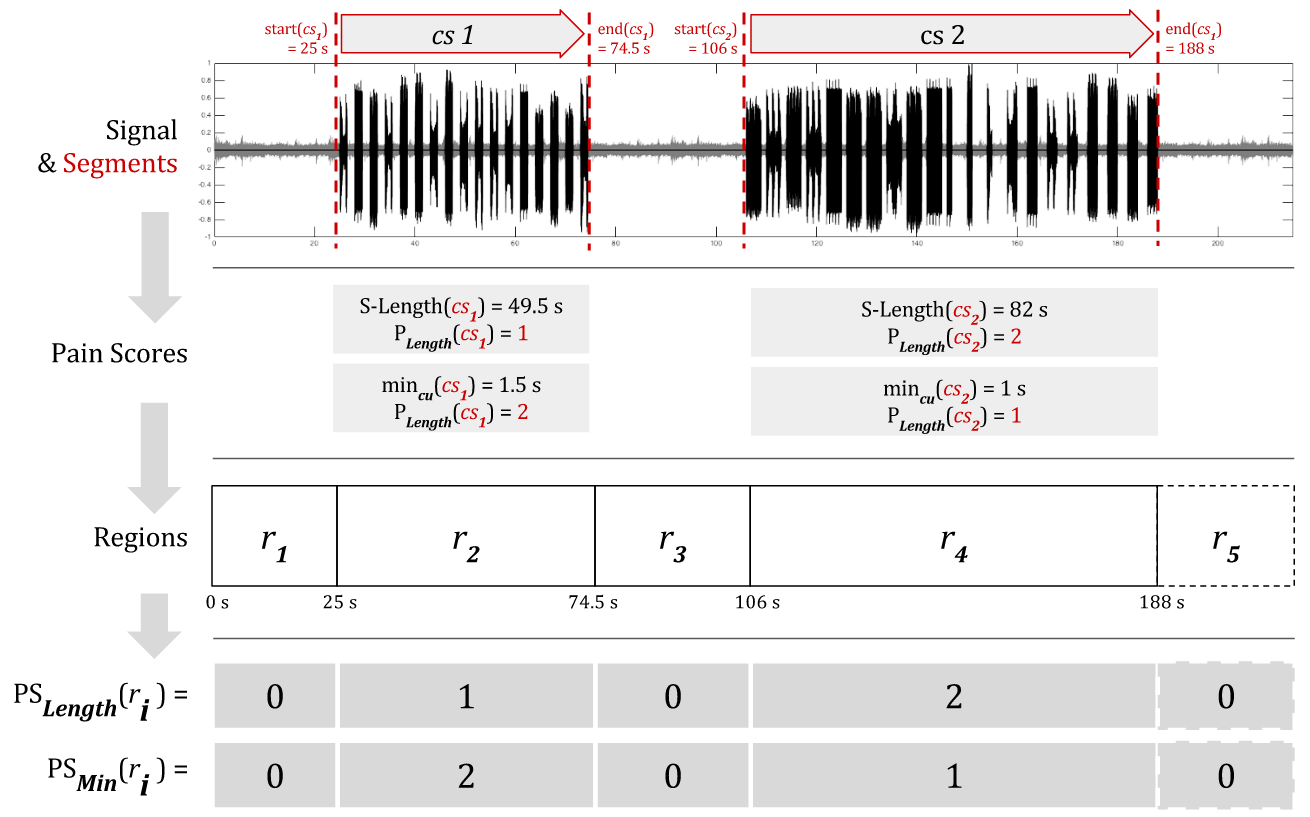
\includegraphics[width=1\textwidth]{bilder/visualisation_example_01.png}
	\caption{Oben: Ein Beispielsignal mit zwei Segmenten, die mit $t_s = \SI{10}{\second}$ gefunden wurden. Darunter: Pain Scores, die für die beiden Segmente berechnet wurden. Darunter: Schematische Darstellung des Signals als Regionen. Unten: Scores der Regionen.}
	\label{img:visualisation_example_01}
\end{figure}

Die grundlegende Idee der Visualisierung ist, den zeitlichen Verlauf des Signals schematisch als einen \emph{Balken} darzustellen. Dieser Balken wird in \emph{Regionen} eingeteilt. Eine Region $r$ beinhaltet entweder ein Cry-Segment oder den Stillebereich zwischen zwei Cry-Segmenten. Die Länge einer Region entspricht der zeitlichen Länge des jeweiligen Stille- oder Cry-Segments. In Abbildung \ref{img:visualisation_example_01} gibt es fünf Regionen $r_{1} , \ldots , r_5 $, wobei die Region $r_2$ und $r_4$ Cry-Segmente enthalten. Die letzte Region wurde noch nicht abgeschlossen, da angenommen wird, dass das Signal weiterhin kontinuierlich eingelesen wird.

Jeder Region wird ein Pain Score zugewiesen. Enthält die Region ein Segment, so wird der Score des Segmentes für die Region übernommen. Regionen ohne Segment bekommen, unabhängig von der verwendeten Pain Scale, einen Score von 0, wie Gleichung \ref{eq:region_score} definiert. Es wird somit angenommen, dass ein Score von 0 bei jeder Pain Scale den Zustand \glqq kein Schmerz\grqq{} codiert, was zumindest bei allen in Kapitel \ref{tab:painscores} vorgestellten Pain Scales der Fall ist. Abbildung \ref{img:visualisation_example_01} unten visualisiert diese Zuweisung von Scores zu den Regionen.

\begin{equation}
PS_{\text{Scale}}(r) = \begin{cases}
 0 \quad \quad \quad,  \text{wenn } r  \text{ kein Cry-Segment beinhaltet} \\
 PS_{\text{Scale}}(cs) \;, \text{wenn } r  \text{ ein Cry-Segment } cs \text{ beinhaltet}
 \end{cases}	
 \label{eq:region_score}
\end{equation}

Das Ziel ist es nun, jede Region mit einer Farbe einzufärben, die den entsprechenden Score anzeigt. Dazu wird für jede Pain Scale eine Funktion $F_{Scale}:S_{Scale} \mapsto P_{Scale}$ benötigt, welche einen Pain Score auf eine Farbe abbildet. Eine Abbildungsfunktion $F_{Scale}$ wird in diesem Zusammenhang als \emph{Farbschema} bezeichnet und der Funktionsbereich $P_{Scale}$ als \emph{Farbpalette}. Ein Farbschema soll die folgenden Kriterien erfüllen:

\begin{description}
\item[Injektivität] Jeder Score einer Scale soll anhand seiner Farbe eindeutig erkennbar sein. Dementsprechend soll gelten: $|S_{Scale}| \leq |P_{Scale}|$.
\item[Intuitive Farbsemantik durch Ampelschema] Ein Farbschema soll eine intuitive Zuordnung zwischen der Höhe des Score und der jeweiligen Farbe ermöglichen. In dieser Arbeit wurde sich für ein Ampelschema entschieden. Das heißt, dass für eine Pain Scale der jeweils niedrigste Score \glqq grün\grqq{}, der höchste Score \glqq rot\grqq{} und ein \glqq mittlerer\grqq{} Score als \glqq leicht rötliches gelb\grqq{} dargestellt wird. Definiert eine Pain Scale einen maximalen Score von 2, so wie beispielsweise das FLACC-System, so ergibt sich die Abbildung $F_{FLACC}(0) =  grün$, $F_{FLACC}(1) = gelb$, $F_{FLACC}(2) = rot$. Definiert die Pain Scale mehr Scores, wie beispielsweise das MBPS mit ingesamt fünf möglichen Scores, so müssen geeignete Zwischenfarben definiert werden. Daraus folgt, dass zwei Pain Scales, deren Menge an Scores gleich groß ist, das selbe Farbschema verwenden.
\item[Visuelle Gleichabständigkeit der Farben] Pain Scales definieren die Scores zwar in einer Reihenfolge, gewährleisten aber keine Vergleichbarkeit. Daher sollen die Farben eines Farbschemas eine \glqq visuelle Gleichabständigkeit\grqq{} gewährleisten. Damit ist gemeint, dass die Farben, auf die jeweils zwei aufeinander folgende Scores einer Scale abgebildet werden, visuelle den gleichen Abstand zueinander haben. So wird verhindert, dass ein Farbschema eine Nähe oder einen Abstand zwischen Scores suggeriert, der durch die jeweilige Pain Scale nicht codiert wird. 
\item[Visuelle Gleichwichtigkeit der Farben] Es kann nicht davon ausgegangen werden, dass ein bestimmter Score für die medizinische Fachkraft von größerem Interesse ist als ein anderer Score. Daher soll keine Farbe einer Farbpalette eine besondere Wichtigkeit suggerieren. Dies wird umgesetzt, in dem alle Farben einer Palette mit einer ähnliche Buntheit definiert werden.\cite{bigman}
\end{description}

Das Kriterium der Gleichabständigkeit legt die Verwendung des \emph{CIELAB}-Raum zur Farbdefinition für die Farbpaletten nahe. Der Farbraum ist in Bezug auf die menschliche Farbwahrnehmung \glqq gleichförmig\grqq. Das heißt, dass die euklidische Distanz zwischen zwei Farben im Farbraum ihrer wahrgenommenen Unterschiedlichkeit entsprechen. Da die Farbdefinition im CIELAB-Raum jedoch auf für den Menschen unintuitiven Parametern beruht, wird weiterhin der \emph{LCH}-Raum verwendet, der zylindrischen Transformation des CIELAB-Raumes. Dieser erlaubt die Farbdefinition auf Basis der für den Menschen intuitiveren Parameter \textbf{L}uminance (Luminanz), \textbf{C}hroma (Buntheit) und \textbf{H}ue (Farbton). Dies Erleichtert die Erfüllung der Farbsemantik, da sich die Farben Grün, Gelb und Rot in der H-Dimension des LCH-Raums in direkter Nachbarschaft befinden.\cite{palettes}\cite{johnstone}

Zur Zusammenstellung der konkreten Farbpaletten wird das Unterstützungwertkzeug \glqq Lch and Lab colour and gradient picker\grqq{} von David Johnstone verwendet.\footnote{Online unter: \url{http://davidjohnstone.net/pages/lch-lab-colour-gradient-picker}} Das Tool erlaubt die Wahl von $n$ Farben LCH-Raum, welche im folgenden als \glqq Fixpunkte\grqq bezeichnet werden. Diese werden ihrer Reihenfolge nach als Eckpunkte eines Pfades durch den Farbraum definiert. Auf Basis dieses Pfades generiert das Tool eine Farbpalette mit $m$ Farben. Ist $n = m$, so entspricht die Farbpalette den definierten Fixpunkten. Ist $m > n$, so findet das Tool die Zwischenfarben durch lineare Interpolation auf den Pfadkanten.

Ein \glqq reines Rot\grqq, codiert im RGB-Raum mit $[255,0,0]$, hat im LCH-Raum die Koordinaten $[53,105,40]$. \glqq Reines Grün\grqq{} hat die Koordinaten RGB $=[0,255,0]$, was LCH $= [88,120,136]$ entspricht. Das \glqq leicht rötliche Gelb\grqq wird definiert mit RGB $=[255,240,0] \hat{=}$LCH $= [93,93,99]$. Diese Farben haben im LCH Raum eine unterschiedliche Buntheit, weshalb sie in einer Farbpalette eine unterschiedliche Wichtigkeit suggerieren würden.\cite{bigman} Daher wurde die Buntheit aller drei Fixpunkte auf den niedrigsten der drei Werte, $93$, gesetzt. Die tatsächlichen Parameter der drei Fixpunkte \emph{Rot}, \emph{Gelb} und \emph{Grün} sind Tabelle \ref{tab:fixpoints} zu entnehmen. 

\begin{table}[h]
\centering
\caption{Fixpunkte als Basis der Farbpaletten}
\label{tab:fixpoints}
\begin{tabular}{@{}llll@{}}
\toprule
                                     & L      & C     & H      \\ \midrule
Rot   & 53     & 93    & 40     \\
Gelb  & 93     & 93    & 99     \\
Grün  & 88     & 93    & 136    \\ \bottomrule
\end{tabular}
\end{table}

Abbildung \ref{fig:color-swatches} zeigt die Farbpaletten, die mit Hilfe des Tools für zwei bis sieben Farben auf Basis dieser Fixpunkte erstellt wurden. Bei der Farbpalette mit ungerader Farbanzahl befinden sich die Fixpunkte an der ersten, letzten und mittleren Position, während die zusätzlichen Farben durch Interpolation erzeugt wurden. Bei den Farbpaletten mit gerader Farbanzahl wird der mittlere Fixpunkt, das Gelb, vom Tool entfernt.

\begin{figure}[h]
	\centering
	\includegraphics[width=0.75\textwidth]{bilder/colorpics.png}
	\caption{Erstellte Farbpaletten mit zwei bis sieben Farben inklusive der zugehörigen RGB-Koordinaten im Hex-Code.}
	\label{fig:color-swatches}
\end{figure}

Auf Basis die Farbpaletten wurden die Farbschemen $L_{n}: S_{Scale} \mapsto P_{Scale}$ definiert, abgebildet in Tabelle \ref{tab:color_shemes}. Es gilt $n = |S_{Scale}|$. Die Wahl des Farbschemas zur Visualisierung einer Pain Scale richtet sich also allein nach der jeweiligen Anzahl definierter Pain Scores, also $F_{Scale} = L_{|S_{Scale}|}$. Soll also beispielsweise die \glqq Length-Scale\grqq{} visualisiert werden, so wird das Farbschema $F_{\text{Length-Scale}} = L_3$ verwendet. Ein Pain Score von $s = 0$ wird durch das Grün mit den RGB-Kooridaten $\#6efa56$ codiert, 1 durch \#6efa56 und 2 durch \#6efa56.

Es wurden keine Farbschemen für $n<1$ definiert, da eine Pain Scale mit nur einer Score nicht sinnvoll ist, sowie keine Farbpaletten mit $n>7$, da keine der in Kapitel \ref{sec:painScores} gelisteten Pain Scales mehr als 7 Scores verwendet. Die Farbpaletten der Schemen $S_2, S_3, S_5$ und $S_7$ wurden direkt aus den Farbpaletten mit der jeweiligen Anzahl an Farben übernommen, die mit Hilfe des Tools von David Johnstone erzeugt wurden (Siehe Abbildung \ref{fig:color-swatches}). Die durch das Tool erzeugten Farbpalette mit vier und sechs Farben wurde nicht für die Schemen $S_3$ und $S_6$ übernommen, da in ihr der Gelbe Fixpunkt nicht enthalten war. Stattdessen wurden die jeweils nächst höheren Farbpaletten unter Auslassung des ersten Grüns verwendet. 

\begin{table}[h]
\centering
\caption{Definition der Farbschemen zur Visualisierung der Pain Scales. Die Farbwerte werden als Hexadezimal-Codes für den RGB-Farbraum angegeben. }
\label{tab:color_shemes}
\begin{tabular}{@{}clllllll@{}}
\toprule
              $s=$         & $0$                                                     & $1$                                                     & $2$                                                     & $3$                                                     & $4$                                                     & $5$                                                     & $6$                                                     \\ \midrule
\multicolumn{1}{l|}{$L_2(s) = $} & \multicolumn{1}{l|}{\cellcolor[HTML]{6EFA56}\#6efa56} & \multicolumn{1}{l|}{\cellcolor[HTML]{F32D16}\#f32d16} &                                                       &                                                       &                                                       &                                                       &                                                       \\ \cmidrule(lr){2-4}
\multicolumn{1}{l|}{$L_3(s) = $} & \multicolumn{1}{l|}{\cellcolor[HTML]{6EFA56}\#6efa56} & \multicolumn{1}{l|}{\cellcolor[HTML]{FFF000}\#fff000} & \multicolumn{1}{l|}{\cellcolor[HTML]{F32D16}\#f32d16} &                                                       &                                                       &                                                       &                                                       \\ \cmidrule(lr){2-5}
\multicolumn{1}{l|}{$L_4(s) = $} & \multicolumn{1}{l|}{\cellcolor[HTML]{B6F52B}\#bff729} & \multicolumn{1}{l|}{\cellcolor[HTML]{FFF000}\#fff000} & \multicolumn{1}{l|}{\cellcolor[HTML]{F98E0B}\#ff9900} & \multicolumn{1}{l|}{\cellcolor[HTML]{F32D16}\#f32d16} &       &                                                       &                                                       \\ \cmidrule(lr){2-6}
\multicolumn{1}{l|}{$L_5(s) = $} & \multicolumn{1}{l|}{\cellcolor[HTML]{6EFA56}\#6efa56} & \multicolumn{1}{l|}{\cellcolor[HTML]{BFF729}\#bff729} & \multicolumn{1}{l|}{\cellcolor[HTML]{FFF000}\#fff000} & \multicolumn{1}{l|}{\cellcolor[HTML]{F98E0B}\#ff9900} & \multicolumn{1}{l|}{\cellcolor[HTML]{F32D16}\#f32d16} &                                                       &                                                       \\ \cmidrule(lr){2-7}
\multicolumn{1}{l|}{$L_6(s) = $} & \multicolumn{1}{l|}{\cellcolor[HTML]{A7F938}\#a7f938} & \multicolumn{1}{l|}{\cellcolor[HTML]{D5F519}\#d5f519} & \multicolumn{1}{l|}{\cellcolor[HTML]{FFF000}\#fff000} & \multicolumn{1}{l|}{\cellcolor[HTML]{FFB700}\#ffb700} & \multicolumn{1}{l|}{\cellcolor[HTML]{FF7A00}\#ff7a00} & \multicolumn{1}{l|}{\cellcolor[HTML]{F32D16}\#f32d16} &                                                       \\ \cmidrule(l){2-8} 
\multicolumn{1}{l|}{$L_7(s) = $} & \multicolumn{1}{l|}{\cellcolor[HTML]{6EFA56}\#6efa56} & \multicolumn{1}{l|}{\cellcolor[HTML]{A7F938}\#a7f938} & \multicolumn{1}{l|}{\cellcolor[HTML]{D5F519}\#d5f519} & \multicolumn{1}{l|}{\cellcolor[HTML]{FFF000}\#fff000} & \multicolumn{1}{l|}{\cellcolor[HTML]{FFB700}\#ffb700} & \multicolumn{1}{l|}{\cellcolor[HTML]{FF7A00}\#ff7a00} & \multicolumn{1}{l|}{\cellcolor[HTML]{F32D16}\#f32d16} \\ \bottomrule
\end{tabular}
\end{table}

Abbildung \ref{fig:viz_without_t_01} zeigt die Visualisierung der Schmerzdiagnostik für das Beispielsignal mit der \glqq Length-Scale\grqq{} und der \glqq Min-Scale\grqq{}, die durch das Einfärben der in Abbildung \ref{img:visualisation_example_01} erläuterten Regionen entsteht. Wie bereits erläutert, verwendet die \glqq Length-Scale\grqq{} das Farbschema $L_3$. Die \glqq Min-Scale\grqq{} definiert insgesamt 4 Scores und verwendet somit das Farbschema $L_4$.

\begin{figure}[h]
	\centering
	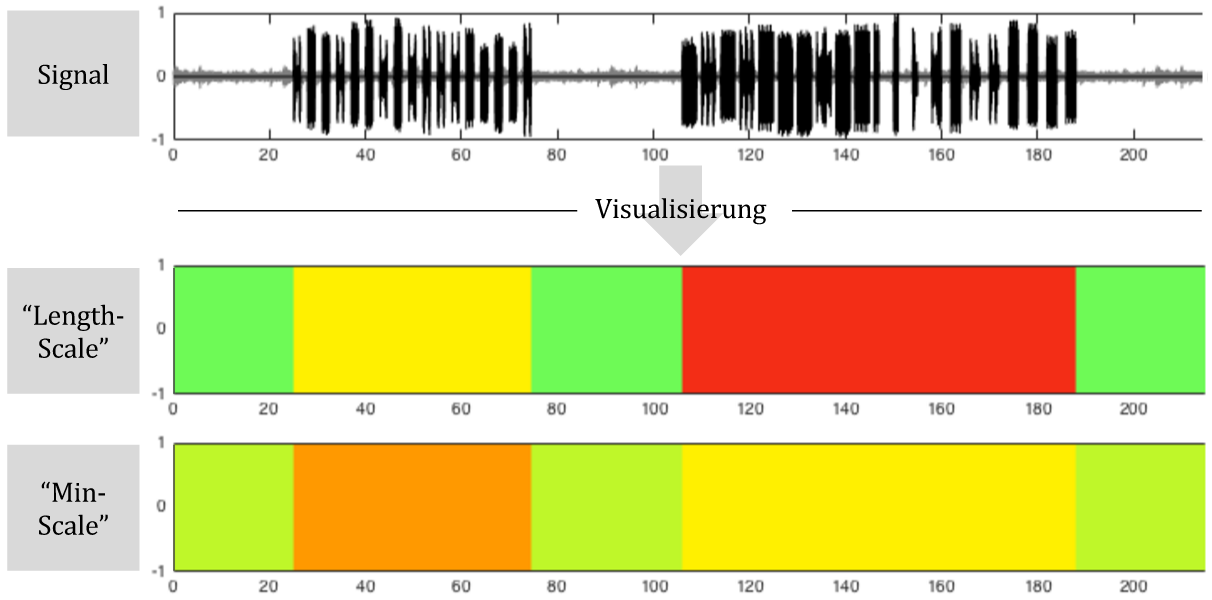
\includegraphics[width=1\textwidth]{bilder/viz_without_t_02.png}
	\caption{Visualisierung der \glqq Length-Scale\grqq{} und der \glqq Min-Scale\grqq{} für das Beispielsignal. }
	\label{fig:viz_without_t_01}
\end{figure}

Da in diesem Beispiel kein Aktualisierungsintervall eingesetzt wurde, gibt es keine überlappenden Regionen. Abbildung \ref{fig:viz_multiple_regions} veranschaulicht, wie durch die Verwendung eines Aktualisierungsintervalls überlappende Regionen entstehen. Oben in der Abbildung ist das Beispielsignal zu sehen, welches mit $t_s = \SI{10}{\second}$ segmentiert wurde. Es wurde ein Aktualisierungsintervall von  $t_{act} = \SI{20}{\second}$ und $t_{obs} = \infty$ verwendet. Die Aktualisierungszeitpunkte sind durch kleine Pfeilge angegeben. Unten sind die aus den Subsegmenten entstandenen, einander überlappenden Regionen abgebildet. Für jede Region wir der Score angegeben, der sich nach der Diagnostik der Min-Scale ergibt, sowie jede Region nach dem Schema $L_4$ eingefärbt.

\begin{figure}[h]
	\centering
	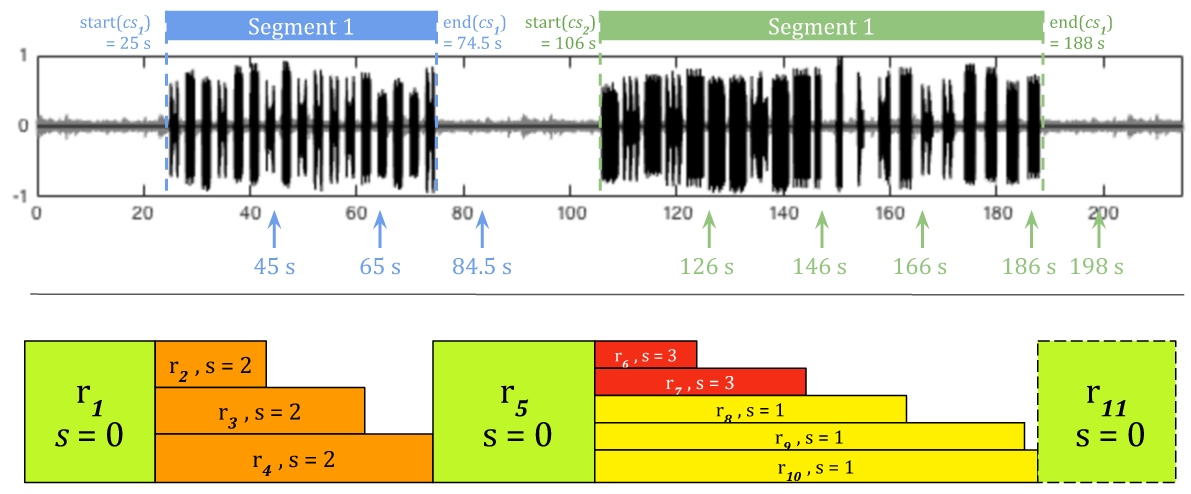
\includegraphics[width=1\textwidth]{bilder/viz-multiple-regions.png}
	\caption{Oben: Beispielsignal mit zwei Segmenten. Unten: Überlappende Regionen, eingefärbt nach dem Farbschema der Min-Scale.}
	\label{fig:viz_multiple_regions}
\end{figure}

Die Darstellung aus Abbildung \ref{fig:viz_multiple_regions} dient nur der Veranschaulichung des Prinzips der überlappenden Regionen, eignet sich aber nicht für eine tatsächliche Visualisierung. Es werden zwei Möglichkeiten zur Visualisierung einander überlappender Regionen vorgeschlagen:
\begin{itemize}
\item Die Region mit dem späteren Endzeitpunkt wird \glqq auf\grqq{} die Regionen mit einem früheren Endzeitpunkt gelegt. So wird der aktuell diagnostizierte Score wird in den Vordergrund gestellt, der zeitliche Verlauf der abgeleiteten Schmerz Scores geht jedoch verloren. Abbildung \ref{fig:viz_act_over} zeigt dieses Prinzip an einem Beispiel. In diesem Fall wurde das Beispielsignal erst bis zu Sekunde $146$ eingelesen, das zweite Segment ist noch geöffnet. Bei der Aktualisierung zum Zeitpunkt $t=\SI{146}{\second}$ wird nach der Min-Scale ein Score von 3 abgeleitet und die Region dementsprechend rot eingefärbt. Das Signal wird nun weiter eingelesen. Bei der nächsten Aktualisierung bei $t=\SI{166}{\second}$ wird ein Score von 1 abgeleitet und die so gelb gefärbte Region \glqq auf\grqq die rot gefärbte Region gelegt.

\begin{figure}[h]
	\centering
	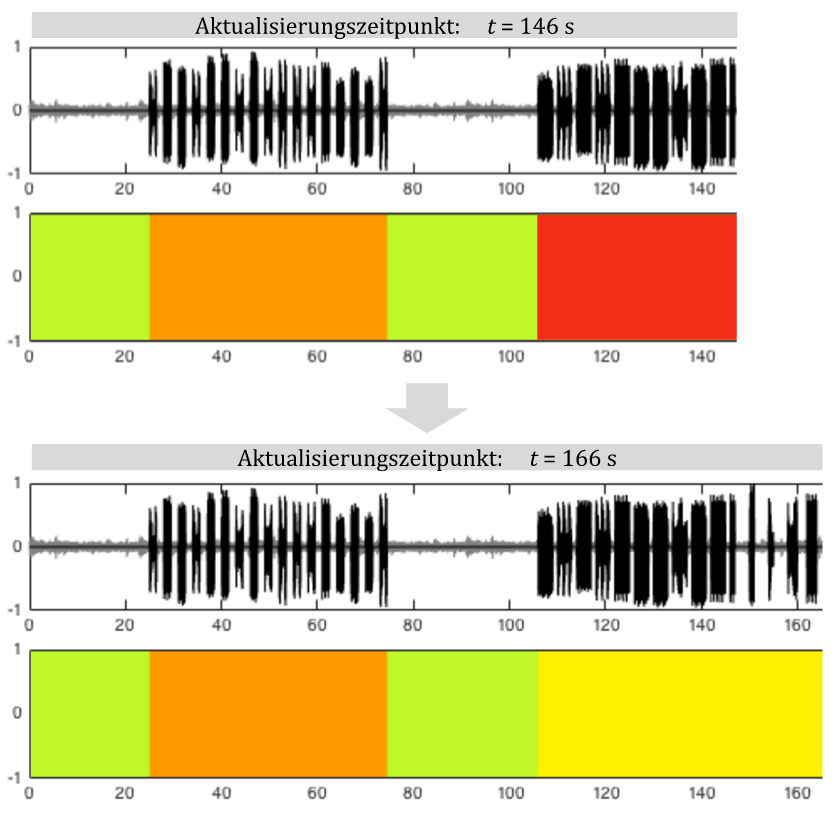
\includegraphics[width=0.7\textwidth]{bilder/viz_act_over.png}
	\caption{Visualisierung der Schmerzdiangostik mit der Min-Scale bei Aktualisierungen. Die aktuellere Region wird \emph{über} ältere Regionen gelegt.}
	\label{fig:viz_act_over}
\end{figure}

\item Die Region mit dem späteren Endzeitpunkt wird \glqq unter\grqq{} die Regionen mit einem früheren Endzeitpunkt gelegt. So wird der zeitliche Verlauf des diagnostizierten Schmerzes in den Vordergrund gestellt. Abbildung \ref{fig:viz_act_under} zeigt die Visualisierung der Schmerzdiagonstik mit der Min-Scale nach diesem Prinzip. Wie zu sehen ist, bleibt auch nach Aktualisierung der Schmerzscore des zweiten Segmentes auf 1 erkennbar, dass bei der früheren Aktualisierung ein Score von 3 abgeleitet wurde.

\begin{figure}[h]
	\centering
	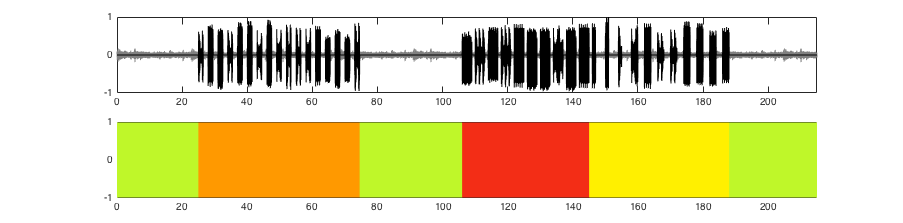
\includegraphics[width=1\textwidth]{bilder/viz_act_under.png}
	\caption{Visualisierung der Schmerzdiangostik mit der Min-Scale bei Aktualisierungen. Die aktuellere Region wird \emph{unter} ältere Regionen gelegt.}
	\label{fig:viz_act_under}
\end{figure}
 
\end{itemize}
